\subsection{Two HOGs Features vector}
After exploring different combinations of $split\times bin\_size$ we wanted to explore the possibilities of creating features vector the comprised from two HOGs. For our experiment we created different combinations of $split\times bin\_size$ and comprised the into one vector, later we used the "Linear Kernel" to check the performance of the different combination. In figure[\ref{fig:exp1a}] we can see the performance of our classifier. The numbers the axis stands for hog configuration ($HOG(Split\_Bins)$) and the gradient of color stands for the accuracy(\textbf{Note}: the darker blue, the better accuracy). 
\begin{figure}[!h]
    \centering
    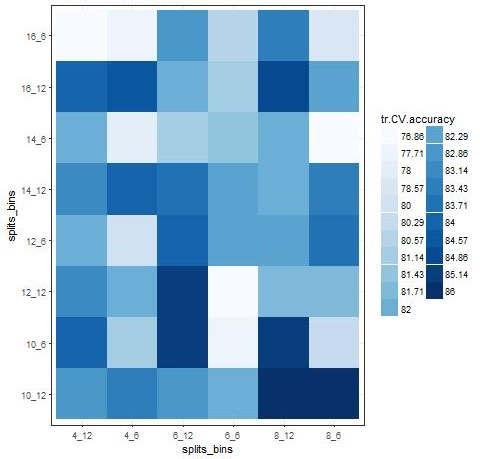
\includegraphics[width=0.6\textwidth]{Images/Accuracy_for_categories_1a.jpeg}
    \caption{Accuracy of Split and Bin combination with linear kernel}
    \label{fig:exp1a}
\end{figure}

From figure[\ref{fig:exp1a}] we can learn, again, that it's hard to draw conclusions for the "right" combination.
\begin{itemize}
    \item Two combinations get 86\% accuracy: $F_1: (8\_6, 10\_12)$ and $F_2: (8\_12,10\_12)$
    \item Three combination get 85.14\% accuracy: $F_3:(6\_12, 10\_6)$, $F_4:(8\_12, 10\_6)$ and \\ $F_5:(6\_12, 12\_12)$
\end{itemize}

Our intuition from the experiment is that HOG with big bin (=12) will be work better with both big and big bin. In case HOG with big bin combined with Hog with small bin, the small bin should have relative high split. This intuition can be used only as \textit{rule of thumb} as we can see, for example, the combination of $HOG(14\_12)$ with $HOG(8\_6)$ perform better than with $HOG(6\_8)$, however, the combination with $HOG(4\_6)$ outperform the bigger split.

The conclusion from the experiment is that in order to get better quality features vector combination we need to apply more complicated technique such as "Spatial Pyramid Matching" as suggested in \cite{Spatial_Pyramid}. Since extending the features vector is costly in power computing (for our poor laptops) and the performance just slightly improved, we decided to to stick with one HOG as features vector.